\begin{figure}

\begin{center}
\begin{subfigure}[b]{\linewidth}
\begin{minipage}{0.5\linewidth}

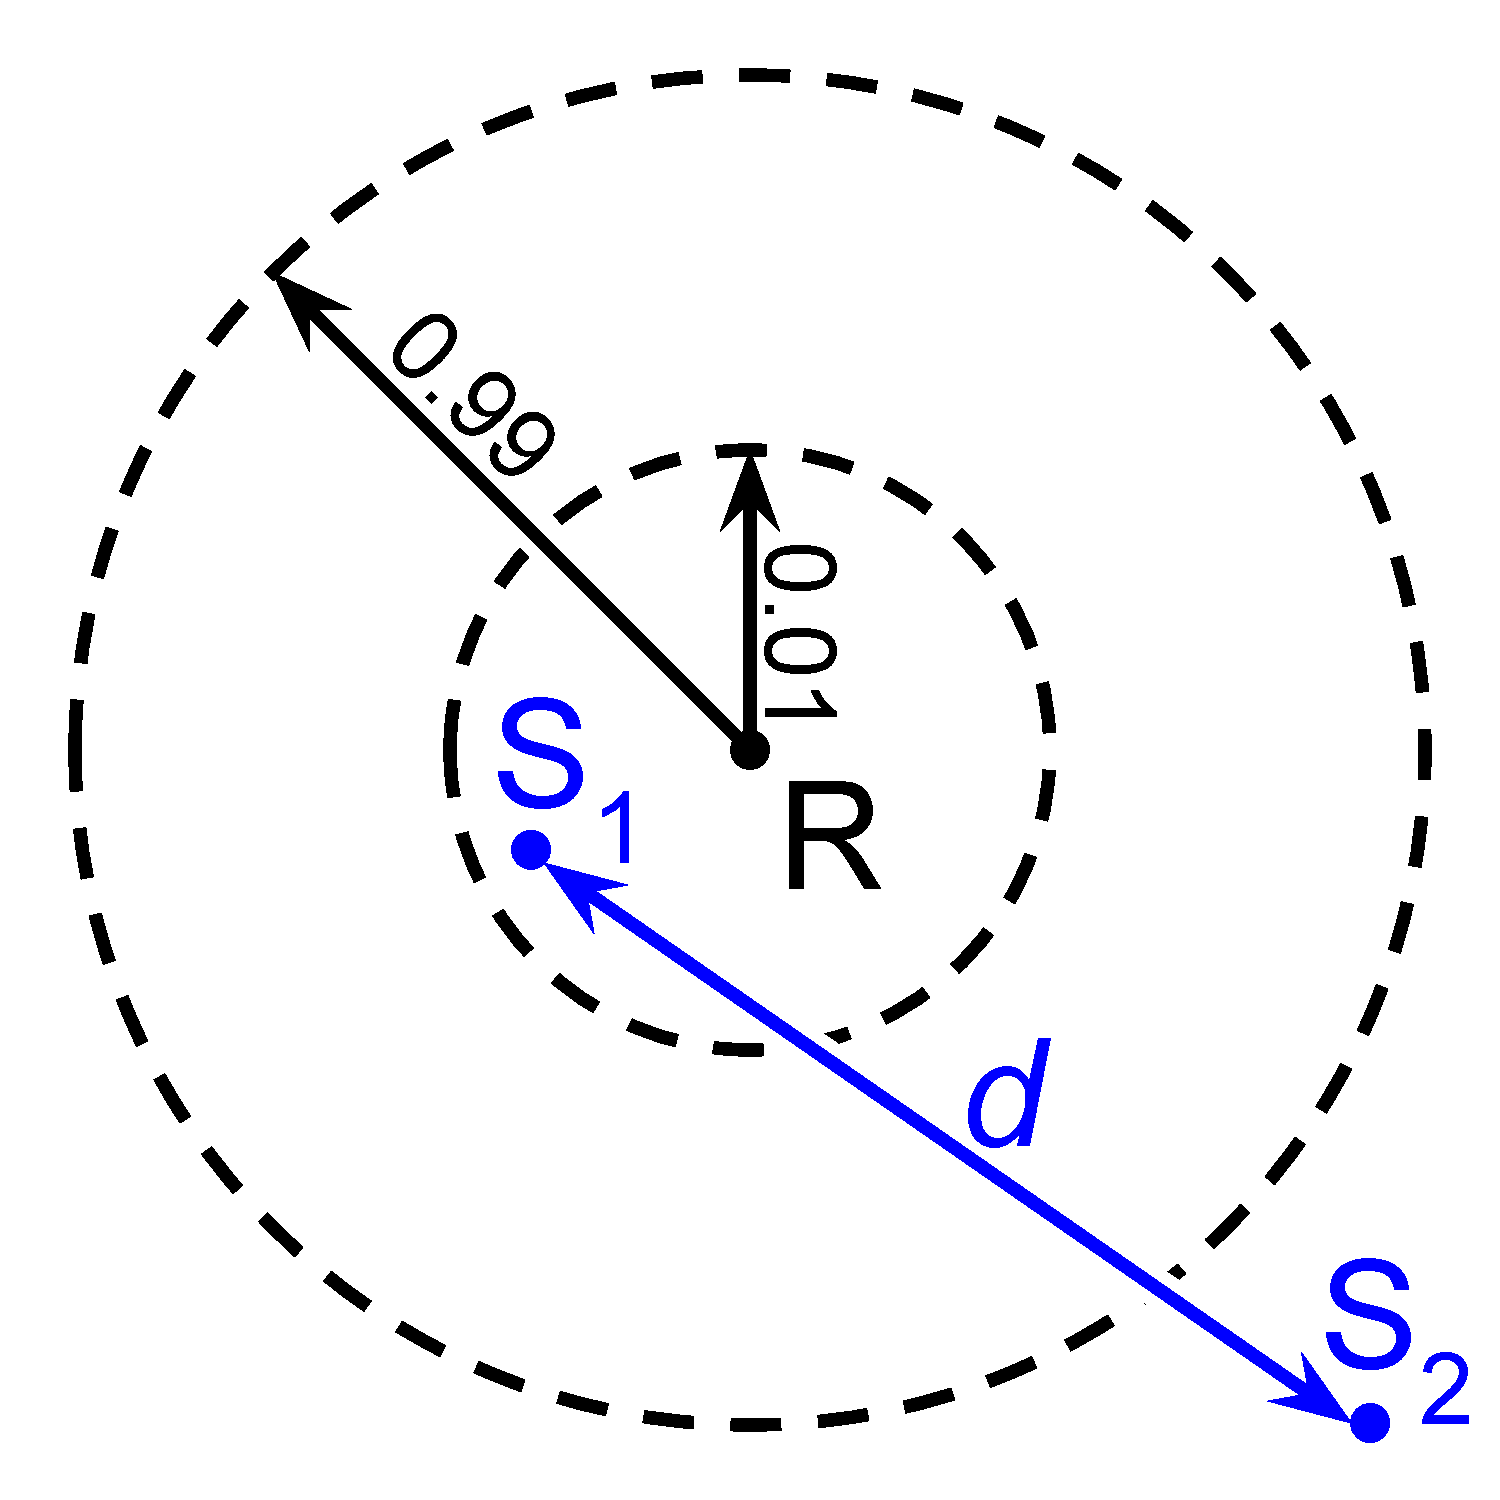
\includegraphics[width=0.75\linewidth]{img/elasticity-statistic}

\end{minipage}
\begin{minipage}{0.5\linewidth}
\caption{
Sampling process used to measure dissimilarity constraint.
First, a constraining tag $R$ was randomly sampled.
Then, tags were randomly drawn until a tag $S_1$ with distance to $R$ less than 0.01 was obtained.
Next, tags were randomly drawn until a tag $S_1$ with distance to $R$ more than 0.99 was obtained.
Finally, dissimilarity constraint was measured as the distance $d$ between $S_1$ and $S_2$.
}
\label{fig:dissimilarity_statistic}
\end{minipage}

\end{subfigure}

\begin{subfigure}[b]{\linewidth}
\begin{minipage}{0.6\linewidth}
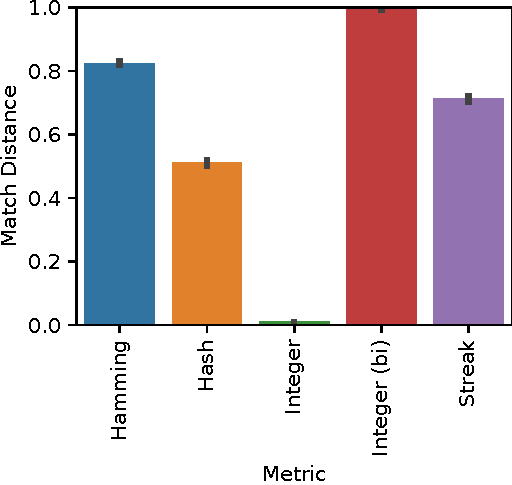
\includegraphics[width=\linewidth]{img/sphere_reverse/bitweight=0dot5+seed=1+title=dimensionality_barplot+_data_hathash_hash=93f97a11cb443d35+_script_fullcat_hash=03ce1e318a24a109+ext=}
\end{minipage}
\begin{minipage}{0.35\linewidth}
\caption{
Mean dissimilarity constraint values for each metric.
Error bars represent 95\% confidence intervals.
}
\label{fig:sphere_reverse_distnplot}
\end{minipage}
\end{subfigure}
\begin{subfigure}[b]{\columnwidth}
\centering
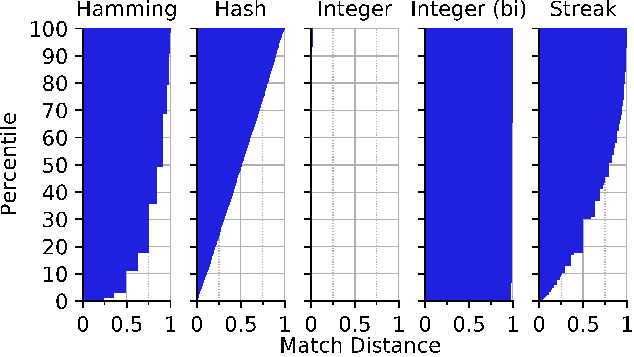
\includegraphics[width=\columnwidth]{img/sphere_reverse/bitweight=0dot5+seed=1+title=dimensionality_distnplot+_data_hathash_hash=93f97a11cb443d35+_script_fullcat_hash=bea2a31376bf6bd0+ext=}
\caption{
Distributions of sampled dissimilarity constraint values.
Each visualization arranges individually sampled observations (thin horizontal bars) vertically in descending order.
The $y$ axis can be interpreted as ranging form the \nth{0} percentile of outcomes (bottom) to \nth{100} percentile (top) with horizontal bar width showing dissimilarity constraint at a certain percentile.
}
\label{fig:sphere_reverse_barplot}
\end{subfigure}

\caption{
Dissimilarity constraint of tag-matching metrics.
Figure \ref{fig:dissimilarity_statistic} summarizes the sampling process used to measure similarity constraint.
Figures \ref{fig:sphere_reverse_barplot} and \ref{fig:sphere_reverse_distnplot} compare distributions of similarity constraint across metrics.
}
\label{fig:sphere_reverse}

\end{center}
\end{figure}
